%
% Main document
%

%
% Styles and packages
%

% !TEX root = ./main.tex

%\documentclass[10pt,a4paper]{report}
\documentclass[11pt,paper=a4,bibliography=totocnumbered,listof=numbered,DIV=calc,oneside,captions=tableheading,headinclude]{scrbook}
%footinclude

\usepackage[utf8]{inputenc}
\usepackage[left=2cm,right=2cm,top=2cm,bottom=2cm]{geometry}

\usepackage[swissgerman]{babel}

\usepackage{amsmath}
\usepackage{amsfonts}
\usepackage{amssymb}
\usepackage{array}
\usepackage{color}
\usepackage[T1]{fontenc}
\usepackage{float}
\usepackage{geometry}
\usepackage{graphicx}
\usepackage{helvet}
\usepackage{hyperref}
\usepackage{hyphsubst}
\usepackage{listings}
\usepackage{lmodern}
\usepackage{makeidx}
\usepackage[numbers]{natbib}
\usepackage{pdfpages}
\usepackage{qtree}
\usepackage{rotating}
\usepackage{tabularx}
\usepackage{url}
\usepackage{wallpaper}

% dev dependency
\usepackage{lipsum}


\begin{document}

  \title{Design von artifiziellen Tieren mit evolutionären Algorithmen}
  \author{Fabian Hediger \and Florian Tanner}
  \date{\today}

  \frontmatter

  %
% Cover page
%

% !TEX root = ./main.tex

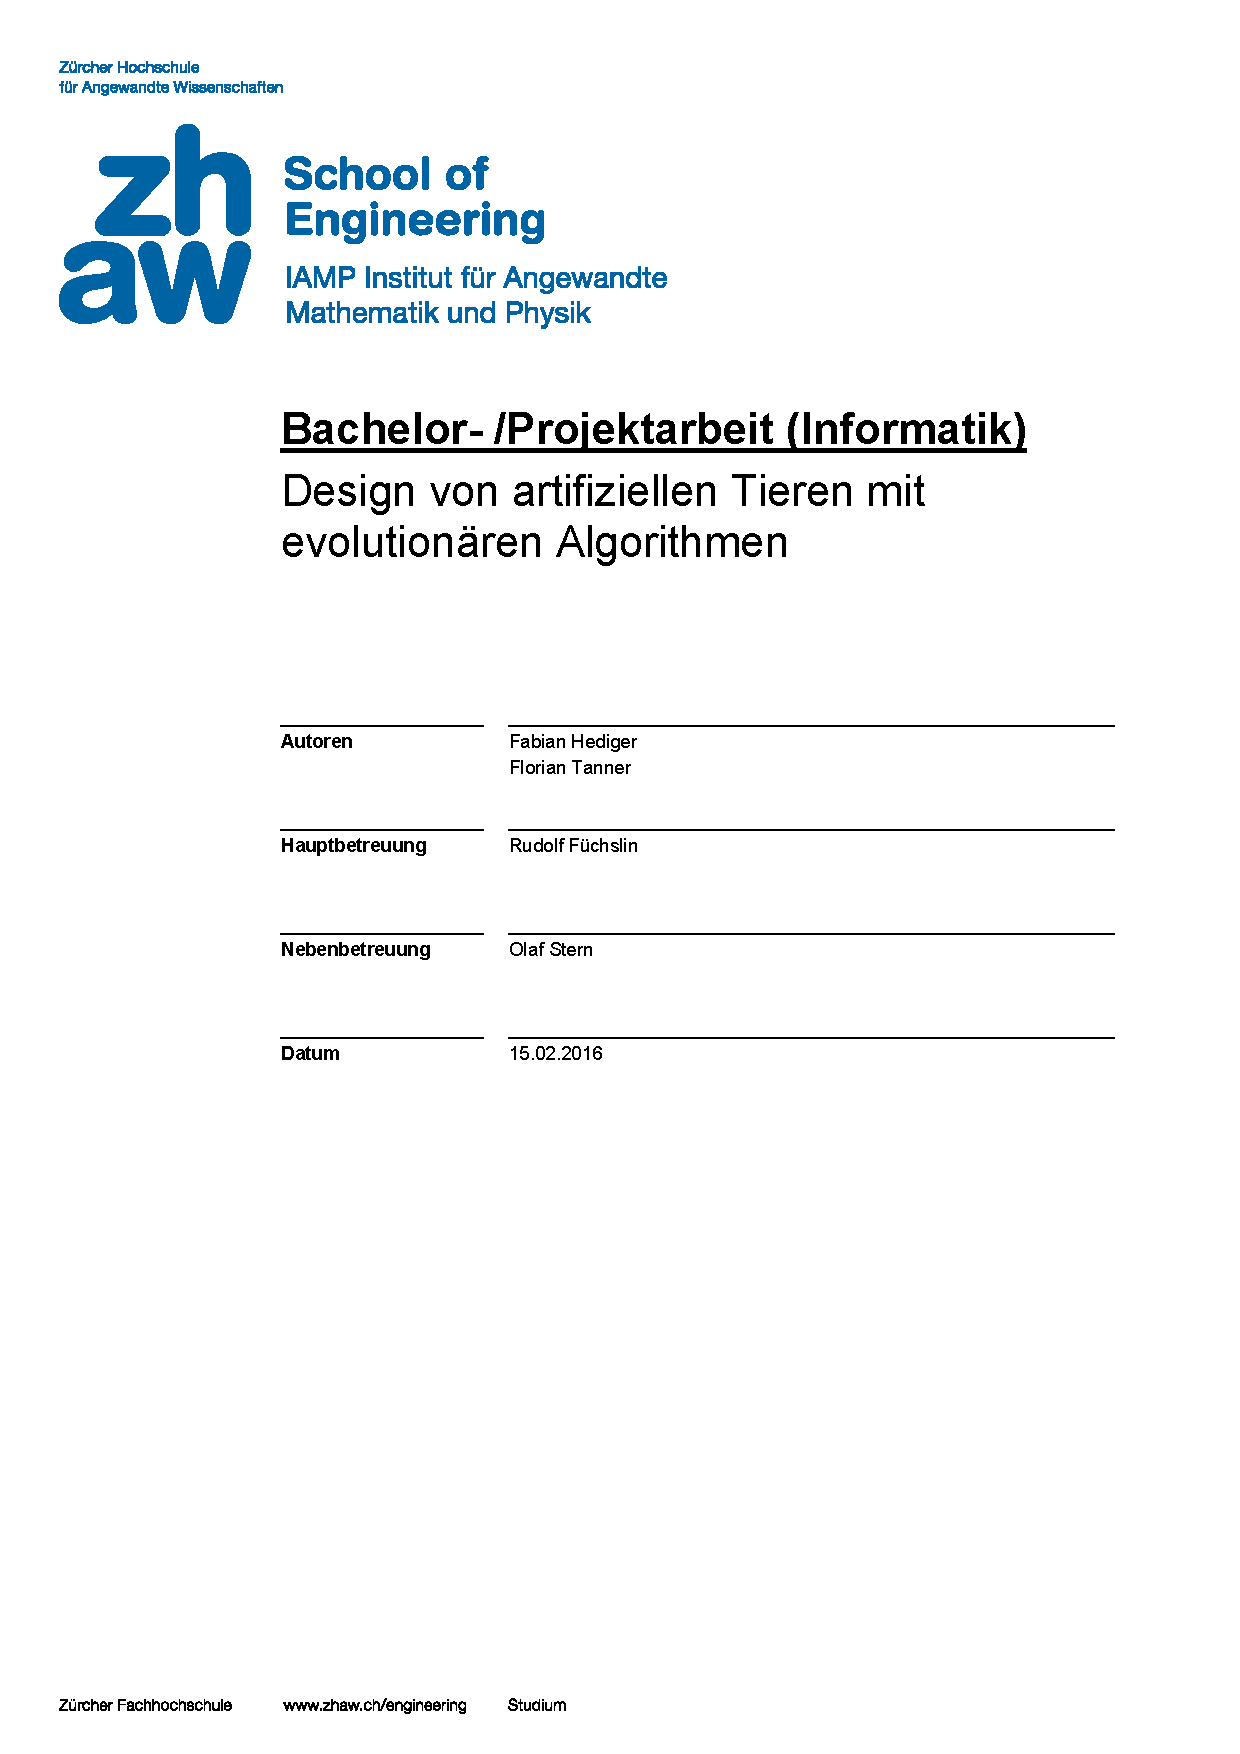
\includepdf{./SoE-IAMP_Bachelor-Titelblatt-Evolut.pdf}
\setcounter{page}{1}

  %
% Table of content
%

% !TEX root = ./main.tex

\tableofcontents
\newpage
\setcounter{page}{1}


  \chapter{Erklärung}
    \lipsum[1]

  \chapter{Vorwort}

    Muss noch übersetzt werden, vieleicht auch nicht im Vorwort, aber ich denke kurzer (oder langer) Theorie Input gut sein.

    \section{Natural Evoltions vs Artifical}
      Natürliche Evolution hat kein vordefiniertes Ziel und ist ein sogennanter \grqq{} open-ended \grqq{} Anpassungsprozess. Artifizielle Evolution jedoch ist ein Optimierungsprozess, welcher versucht Lösungen zu vordefinierten Problem zu finden \cite[S.1]{book:bioInspired}. \\

    \section{Genotype}
      The genetic material of an individual is known as the genotype, whereas its manifestation as an organism is known as the phenotype. Cells contain a class of molecules, known as proteins, whose shape,
      concentration, and behavior determine the properties of the cell. For example hair cells and muscle cells are different because they are composed of different proteins. \\
      The definition of specific proteins depends on another molecule, known as DNA (deoxyribonucleic acid), which in turn relies on proteins to become operative and on the mediation of a third type of molecule,
      known as RNA (ribonucleic acid), which is structurally similar to the DNA molecule. The DNA is the genetic material that is transmitted over generations.
      It is often enclosed within the nucleus of the cell and all cells in the organism have the same genetic material. \\
      DNA molecules are long chains of complementary strands composed of four types of chemical units(nucleotides or bases): adenine (A), cytosine (C), guanine (G), and thymine(T). \\
      The two strands stick together because nucleotides can lock to each other: Adenine binds to thymine and cytosine binds to guanine. This specific binding means that the two DNA strands are perfectly complementary. \\
      The genetic material is organized in several separated DNA molecules, called chromosomes. There are two types of cell replication: mitosis and meiosis. \\
      Mitosis occurs during growth of the organism when a cell divides by producinga copy with the same number of chromosomes (23 times 2 in humans).
      During mitosis, the two strands of the 46 DNA molecules are separated and each strand goes to one cell. Each strand then rebuilds the missing strand by recruiting the complementary nucleotides.
      The process ends with two exact copies of the double-stranded DNA molecule, one for each cell.
      Meiosis occurs during the production of sex cells (sperm and eggs). Sex cells receive only one chromosome for each pair. \\
      In diploid organisms the pairs of chromosomes are recombined during fecundation of the egg cell (containing the set of chromosomes from the mother) by the sperm cell (containing the set of chromosomes from the father).
      \cite[S.5 - 7]{book:bioInspired}.

    \section{Gene Expression}
      The sequence of four nucleotides along the DNA chain determines the properties of the cells and the development of the organism. The four nucleotides are effectively the letters of the genetic alphabet.
      Genes are functionally relevant subsequences of nucleotides in the DNA chain (just like words in a sentence), which can produce proteins.
      Proteins are long molecular chains composed of hundreds of submolecules, known as amino acids.  The properties of a protein are determined mainly by its shape. Each amino acid corresponds to one or
      more specific sequences of three nucleotides (codon) in the DNA chain. The production of proteins \ref{pic:dnaTranscription} from DNA is mediated by RNA.
      RNA is a long molecule similar to DNA, but it consists of only one strand of nucleotides, is much shorter (typically a few thousand nucleotides), and features uracil (U) in place of DNA thymine (T).
      During protein production, the two strands of DNA are separated and an RNA molecule is assembled along a small part of the DNA strand so as to match the corresponding nucleotides.
      This process is known as transcription. The resulting RNA molecule is used to create a protein by assembling a chain of amino acids that correspond to the sequence of nucleotides.
      Some proteins regulate cell division and genetic expression of proteins. It is important to notice that while the sequence of DNA nucleotides cannot be modified by proteins, the sequence of protein amino
      acids is instead determined by DNA. In other words, information flows in one direction only, from genes to proteins. This is the reason why modifications of the phenotype that occur during the life of the individual and are
      caused by environmental phenomena cannot directly modify the genotype and be inherited by offspring (with the exception of exposure to radiation, which can directly affect the DNA sequence).
      \begin{figure}
        \centering
        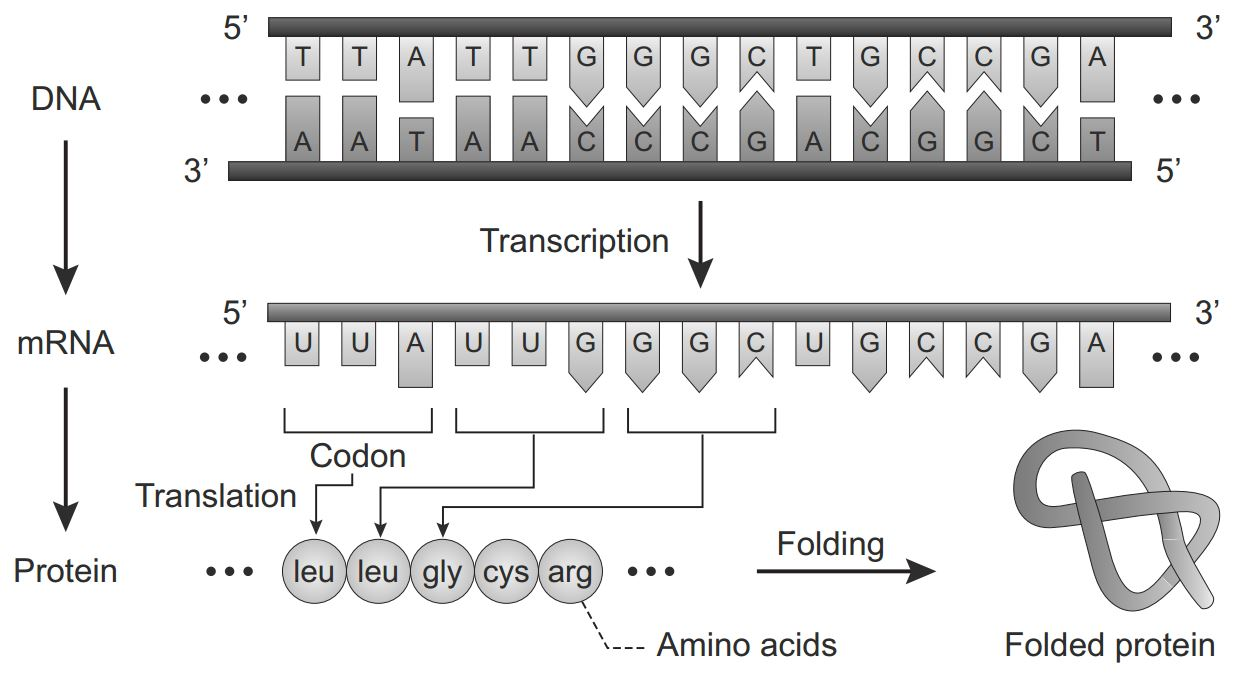
\includegraphics[width=10cm]{graphics/DNA_Transcription_Protein}
        \caption[DNA Transcription]{DNA Transcription Prozess}
        \label{pic:dnaTranscription}
      \end{figure}
  \chapter{Abstract}
    \lipsum[3]

  \mainmatter

  \chapter{Einleitung}
  \lipsum[4-5]
  \section{Thema}
  \lipsum[5-6]

  \chapter{Theorie}
  \lipsum[6] \cite{IEEEexample:article_typical}
  \lipsum[7] \cite{mirrorcle_userguide}

  \chapter{Methode}
  \lipsum[8] \cite{microchip_spi} \cite{verryUseFulArticle}

  \chapter{Resultate}
  \lipsum[9]

  \appendix
  \chapter{Anhang}
  \section{Erster Anhang}

  \backmatter
  %
% Bibliography
%

% !TEX root = ./main.tex

\nobibliography*
\bibliographystyle{IEEEtranN}
\bibliography{IEEEabrv,literature}

  %
% Glossary entries
%

% !TEX root = ../main.tex

%
% Acronyms
%
\newacronym[see={FiniteStateMachine}]{fsm}{EA}{Endlicher Automat}

%
% Entries
%
\newglossaryentry{FiniteStateMachine}
{
  name={Endlicher Automat},
  description={Ein endlicher Automat (Zustandsmaschine, Zustandsautomat) ist ein Modell eines Verhaltens,
    bestehend aus Zuständen, Zustandsübergängen und Aktionen.}
}

\newglossaryentry{Hexapod}
{
  name={Hexapod},
  description={Die Sechsfüßer (griech. Hexapoda) oder Hexapoden
    gehören dem Stamm der Gliederfüßer (Arthropoda) an,
    sie bilden einen Unterstamm von diesen.}
}

\newglossaryentry{JointDriven}
{
  name={joint-driven},
  description={Ein Motor der ``joint-driven'' arbeitet steuert Bewegungen über ein Drehgelenk.
    }
}

\newglossaryentry{SimplePolygon}
{
  name={einfaches Polygon},
  description={Ein einfaches Polygon ist in der Geometrie eine flache Form bestehend aus geraden,
    sich nicht überschneidenden Linien, die einen geschlossenen Pfad formen.}
}

  \listoffigures

\end{document}
